% TODO:
%   - Make this background chapter
%   - Section on ethics
%   - Split out your own work from literature
%   - Move BCI pipeline to separate chapter
% ----------  
% Questions:
%   - XXX

% https://www.brainlatam.com/blog/wet-dry-active-and-passive-electrodes.-what-are-they-and-what-to-choose-413
% https://www.brainlatam.com/blog/a-brief-introduction-to-eeg-and-the-types-of-electrodes-75

% Goed boek voor sources bci_review_book_chapter

% In a new chapter, reset the GLS to once again use full version in first occurence
\glsresetall

\chapter{Biomedical signals}
\label{ch:biomedical_signals}

% ---------------------------------------------- 

\section{Better understanding the data used by BCIs}
\label{sec:biomedical_signals_why}

% TODO
\lipsum[1-2]

% ---------------------------------------------- 

\section{Origin of brain-signals}
\label{sec:biomedical_signals_origin}

% TODO
\lipsum[1-2]

% - - - - - - - - - -

\subsection{Bioelectricity in the human body}
\label{subsec:biomedical_signals_origin_bioelectricity}

% TODO
\lipsum[1-4]

% - - - - - - - - - -

\subsection{Measurable brain activity}
\label{subsec:biomedical_signals_origin_brain_activity}

% TODO
\lipsum[1-3]


% - - - - - - - - - -

\subsection{Anatomy of the brain}
\label{subsec:biomedical_signals_origin_anatomy_brain}

% TODO
\lipsum[1-4]

% - - - - - - - - - -

\subsection{Neuroplasticity and inter-human variation}
\label{subsec:biomedical_signals_origin_general_brain_layout}

% TODO
\lipsum[1-3]

% ---------------------------------------------- 

\section{Types of brain-signals}
\label{sec:biomedical_signals_type_of_signals}

% TODO
\lipsum[1-2]

% - - - - - - - - - -

\subsection{Brain waves frequencies}
\label{subsec:biomedical_signals_type_of_signals_brain_wave}

% TODO
\lipsum[1-2]

% - - - - - - - - - -

\subsection{Event related potentials}
\label{subsec:biomedical_signals_type_of_signals_erp}

% TODO
% P300 en andere signalen vermeld in introduction
\lipsum[1-2]

% - - - - - - - - - -

\subsection{Motor imagery}
\label{subsec:biomedical_signals_type_of_signals_motor_imagery}

% TODO zie chapter 23 bci_handbook
% Issues MI: https://www.frontiersin.org/articles/10.3389/fnins.2021.824759/full
\Gls{mi} is the process in which a person generates brain-activity in the motor cortex merely by imagining motor movements.
\Gls{mi}-based \glspl{bci} are interesting because they don't require any external stimulus nor effective motor movements

\lipsum[1-3]

% ---------------------------------------------- 


\section{Measuring brain-signals}
\label{sec:biomedical_signals_measuring}

% TODO
\lipsum[1-2]

% ---------------------------------------------- 

\subsection{Measuring modalities}
\label{subsec:biomedical_signals_measuring_modalities}
% EEG ECOG ETC ETC

% TODO
\lipsum[1-5]

Research by \citet{human_eeg_discovery} is the first in describing the measurement of brain waves from the human skull in a non-invasive manner.
Because of this, the German neuroscientist and psychiatrist Hans Berger is often seen as the inventor of \gls{eeg}.
Whilst he was one of the first to use the term \textit{elektrenkephalogramm}, it was Richard Caton who first described the findings of brain waves in general.
He found this phenomena in animal brains as early as 1875 \citep{first_eeg}.
Since then, \gls{eeg} methodology and equipment has matured and evolved a lot.

% - - - - - - - - - -

\subsection{Standardized EEG measuring systems}
\label{subsec:biomedical_signals_measuring_standardization}

% TODO
\lipsum[1-4]

% - - - - - - - - - -

\subsection{Comparison of available EEG measuring equipment}
\label{subsec:biomedical_signals_measuring_equipment}

% TODO
\lipsum[1-5]

% https://imotions.com/blog/eeg-headset-prices/
% Nextmind 
% Neurosky
% Interaxon
% Muse
% Emotiv
% myBrain
% OpenBCI

% TODO: citing for sources of img?
\begin{figure}[ht]
  \begin{minipage}{\textwidth}
    \centering
    \begin{subfigure}{.48\textwidth}
        \centering
        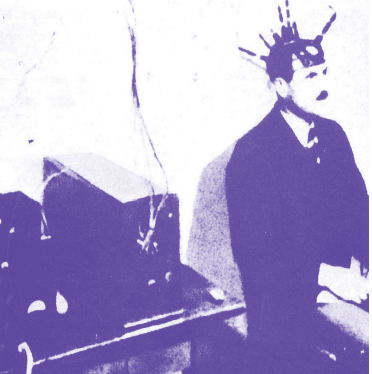
\includegraphics[width=\textwidth]{images/hardware/berger_hardware.png}
        \captionsetup{width=0.9\linewidth}
        \captionsetup{justification=centering}
        \caption{Experimental analog \gls{eeg} recording equipment used by \citet{human_eeg_discovery}.\\Figure by by \citet{oldest_eeg_hardware}.}
        \label{fig:eeg_hardware_evolution_1}
    \end{subfigure}
    \hfill
    \begin{subfigure}{.48\textwidth}
        \centering
        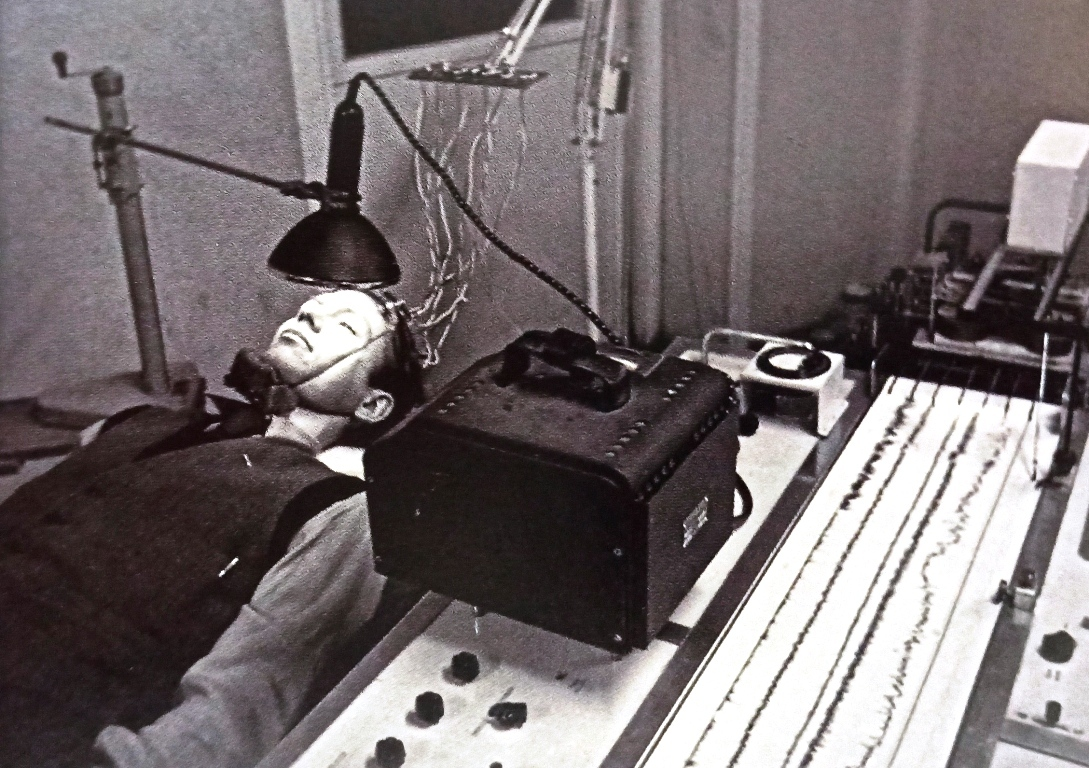
\includegraphics[width=\textwidth]{images/hardware/eeg_1950.jpg}
        \captionsetup{width=0.9\linewidth}
        \captionsetup{justification=centering}
        \caption{Medical-grade analog \gls{eeg} recording equipment estimated to be from the 1950's. \\Figure by Devotor\footnotemark[1].}
        \label{fig:eeg_hardware_evolution_2}
    \end{subfigure}
    \captionsetup{width=0.9\linewidth}
    \bigskip
    \begin{subfigure}{.48\textwidth}
        \centering
        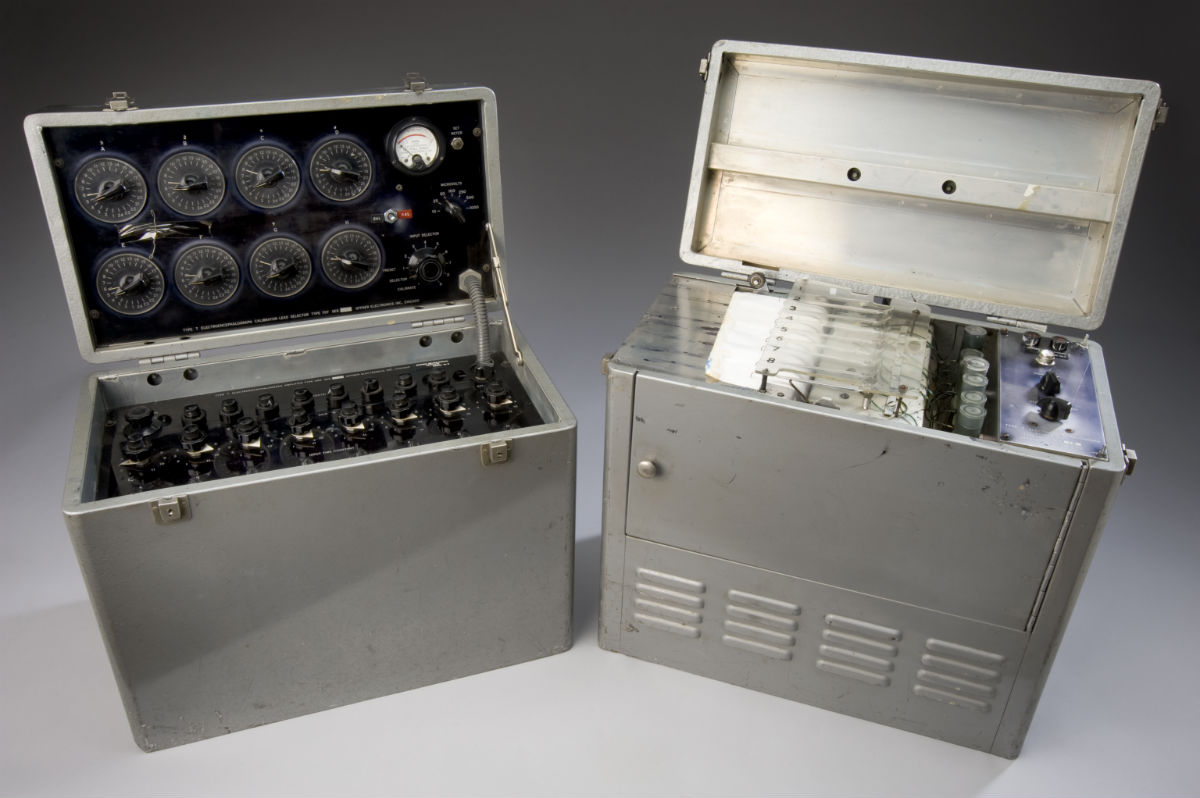
\includegraphics[width=\textwidth]{images/hardware/early_portable_eeg.jpg}
        \captionsetup{width=0.9\linewidth}
        \captionsetup{justification=centering}
        \caption{Early portable analog EEG recording equipment from the late 1950's. \\Figure by Sam Brusco\footnotemark[2]. }
        \label{fig:eeg_hardware_evolution_3}
    \end{subfigure}
    \hfill
    \begin{subfigure}{.48\textwidth}
        \centering
        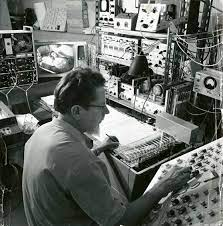
\includegraphics[width=\textwidth]{images/hardware/grey_walter.jpg}
        \captionsetup{width=0.9\linewidth}
        \captionsetup{justification=centering}
        \caption{William Grey Walter and medical-grade analog \gls{eeg} recording equipment, 1964.\\Figure by Burden Neurological Institute\footnotemark[3].}
        \label{fig:eeg_hardware_evolution_4}
    \end{subfigure}
    \captionsetup{width=0.9\linewidth}
    \captionsetup{justification=centering}
    \caption{Early analog \gls{eeg} equipment.}
    \footnotetext[1]{\url{https://www.charismaticplanet.com/the-electroencephalogram-1924/}}
    \footnotetext[2]{\url{https://www.medicaldesignandoutsourcing.com/medtech-memoirs-the-electroencephalograph-eeg/}}
    \footnotetext[3]{\url{http://dx.doi.org/10.15180/181003/019}}
    \label{fig:eeg_hardware_early_analog}
  \end{minipage}  
\end{figure}

% - - - - - - - - - -

\subsection{Usages of invasive systems}
\label{subsec:biomedical_signals_measuring_invasive}

% TODO
\lipsum[1-3]

% - - - - - - - - - -

\subsection{Common EEG artefacts}
\label{subsec:biomedical_signals_measuring_artefacts}

% TODO also discuss how to use them e.g. eye blink as input
\lipsum[1-4]


% ---------------------------------------------- 

\section{Using non-invasive EEG measurements for MI classification}
\label{sec:biomedical_signals_eeg_for_mi_classification}

% TODO
\lipsum[1-2]